\documentclass[aspectratio=169]{beamer}
\usetheme{Madrid}
\usecolortheme{default}

% Packages
\usepackage{listings}
\usepackage{xcolor}
\usepackage{tikz}
\usetikzlibrary{positioning}
\usepackage{pgfplots}
\pgfplotsset{compat=1.18}
\usepackage{amssymb}

% Listings: define YAML (not built-in in many LaTeX setups)
\lstdefinelanguage{yaml}{
  keywords={true,false,null,y,n},
  keywordstyle=\color{blue},
  basicstyle=\ttfamily\small,
  sensitive=false,
  comment=[l]{\#},
  commentstyle=\color{gray},
  stringstyle=\color{red},
  morestring=[b]',
  morestring=[b]"
}

% Code styling (defaults)
\lstset{
  basicstyle=\ttfamily\scriptsize,
  columns=fullflexible,
  keepspaces=true,
  showstringspaces=false,
  breaklines=true,
  breakatwhitespace=true,
  frame=single,
  xleftmargin=0.3em,
  framexleftmargin=0.3em,
  postbreak=\mbox{\textcolor{gray}{$\hookrightarrow$}\space}
}

\title{Angular CI Pipeline Optimization}
\subtitle{From 106s to 62s: A 58\% Performance Improvement}
\author{CI/CD Optimization Report}
\date{\today}

\begin{document}

\frame{\titlepage}

% Slide 1: The Problem
\begin{frame}{The Problem}
\begin{block}{Initial State}
\begin{itemize}
    \item No CI/CD pipeline configured
    \item Using npm (slow package manager)
    \item No caching strategy
    \item No build optimization
    \item No test parallelization
\end{itemize}
\end{block}

\vspace{0.5cm}

\begin{alertblock}{Goal}
Build a highly optimized CI pipeline with aggressive caching to minimize build times and resource usage
\end{alertblock}
\end{frame}

% Slide 2: Performance Results
\begin{frame}{Performance Results}
\centering
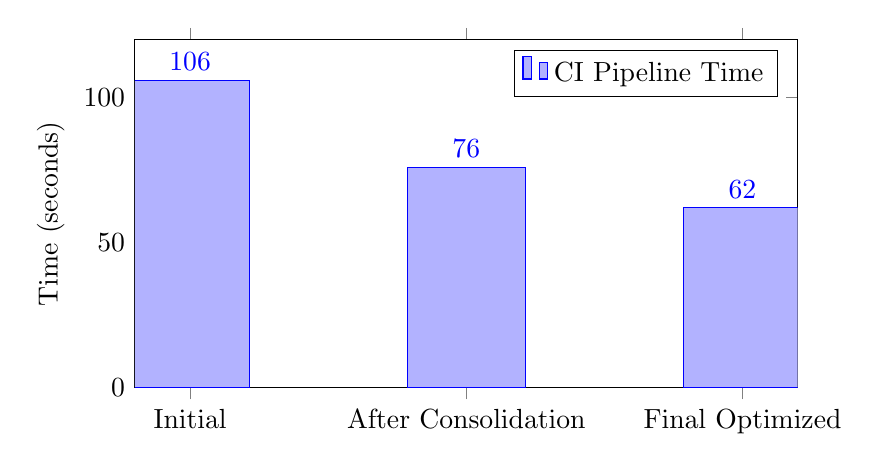
\begin{tikzpicture}
\begin{axis}[
    ybar,
    ylabel={Time (seconds)},
    symbolic x coords={Initial, After Consolidation, Final Optimized},
    xtick=data,
    nodes near coords,
    ymin=0,
    ymax=120,
    width=10cm,
    height=6cm,
    bar width=1.5cm,
    legend pos=north east,
]
\addplot coordinates {(Initial,106) (After Consolidation,76) (Final Optimized,62)};
\legend{CI Pipeline Time}
\end{axis}
\end{tikzpicture}

\vspace{0.3cm}
\textbf{\Large 58\% Faster} \quad $\downarrow$ \textbf{44 seconds saved}
\end{frame}

% Slide 3: Key Optimizations
\begin{frame}{Key Optimizations Implemented}
\begin{columns}[T]
\column{0.5\textwidth}
\textbf{1. Package Manager Migration}
\begin{itemize}
    \item npm $\rightarrow$ pnpm
    \item 40-60\% faster installs
    \item Better disk space efficiency
\end{itemize}

\vspace{0.3cm}

\textbf{2. Dependency Caching}
\begin{itemize}
    \item node\_modules cache
    \item pnpm store cache
    \item 0s installs on cache hit
\end{itemize}

\column{0.5\textwidth}
\textbf{3. Build \& Test Caching}
\begin{itemize}
    \item Angular build cache
    \item Jest transform cache
    \item TypeScript compilation cache
\end{itemize}

\vspace{0.3cm}

\textbf{4. Job Architecture}
\begin{itemize}
    \item Consolidated jobs
    \item Eliminated overhead
    \item Parallel test execution
\end{itemize}
\end{columns}
\end{frame}

% Slide 4: Migration to pnpm
\begin{frame}[fragile]{Migration to pnpm}
\begin{block}{Why pnpm?}
\begin{itemize}
    \item \textbf{Faster}: Hard links instead of copying files
    \item \textbf{Efficient}: Single content-addressable storage
    \item \textbf{Strict}: Better dependency resolution
\end{itemize}
\end{block}

\begin{block}{Configuration}
\begin{lstlisting}[language=bash]
# .npmrc
auto-install-peers=true
store-dir=~/.pnpm-store
lockfile=true
prefer-frozen-lockfile=true
\end{lstlisting}
\end{block}

\textbf{Result}: Install time reduced from 30-40s to \textbf{0s} with cache hit
\end{frame}

% Slide 5: Job Architecture Evolution
\begin{frame}{Job Architecture Evolution}
\begin{columns}[T]
\column{0.48\textwidth}
\textbf{Before: 4 Separate Jobs}

\vspace{0.3cm}

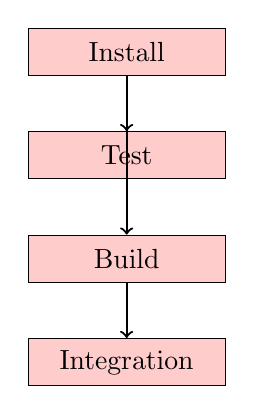
\begin{tikzpicture}[node distance=0.7cm]
\node[draw, rectangle, fill=red!20, minimum width=2.5cm, minimum height=0.6cm] (install) {Install};
\node[draw, rectangle, fill=red!20, minimum width=2.5cm, minimum height=0.6cm, below=of install] (test) {Test};
\node[draw, rectangle, fill=red!20, minimum width=2.5cm, minimum height=0.6cm, below=of test] (build) {Build};
\node[draw, rectangle, fill=red!20, minimum width=2.5cm, minimum height=0.6cm, below=of build] (integration) {Integration};

\draw[->, thick] (install) -- (test);
\draw[->, thick] (install) -- (build);
\draw[->, thick] (build) -- (integration);
\end{tikzpicture}

\vspace{0.3cm}

\textbf{Issues:}
\begin{itemize}
    \item 3x setup overhead
    \item 3x checkout
    \item Cache restore delays
\end{itemize}

\column{0.48\textwidth}
\textbf{After: Unified Job}

\vspace{0.3cm}

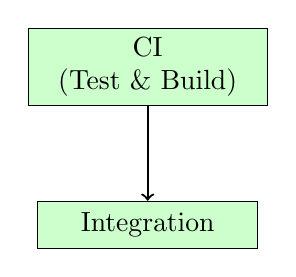
\begin{tikzpicture}[node distance=1.2cm]
\node[draw, rectangle, fill=green!20, text width=2.8cm, align=center, minimum height=0.8cm] (unified) {CI\\(Test \& Build)};
\node[draw, rectangle, fill=green!20, minimum width=2.8cm, minimum height=0.6cm, below=of unified] (integration2) {Integration};

\draw[->, thick] (unified) -- (integration2);
\end{tikzpicture}

\vspace{0.3cm}

\textbf{Benefits:}
\begin{itemize}
    \item 1x setup (saves 60s)
    \item Shared cache
    \item Faster execution
\end{itemize}
\end{columns}
\end{frame}

% Slide 6: Caching Strategy
\begin{frame}{Caching Strategy}
\begin{block}{Three-Layer Cache Approach}

\begin{columns}[T]

\column{0.33\textwidth}
\begin{exampleblock}{1. Dependencies}
\begin{itemize}
  \item node\_modules
  \item pnpm store
  \item Keyed by lockfile
\end{itemize}
\end{exampleblock}

\column{0.33\textwidth}
\begin{exampleblock}{2. Build Artifacts}
\begin{itemize}
  \item Angular cache
  \item TypeScript output
  \item Incremental builds
\end{itemize}
\end{exampleblock}

\column{0.33\textwidth}
\begin{exampleblock}{3. Test Cache}
\begin{itemize}
  \item Jest transforms
  \item Compiled specs
  \item Faster re-runs
\end{itemize}
\end{exampleblock}

\end{columns}

\vspace{0.4cm}

\centering
\textbf{Result:} Zero installs, incremental builds, cached tests on warm runs

\end{block}
\end{frame}


% Slide 7: Test Optimization
\begin{frame}{Test Execution Optimization}
\begin{block}{Parallel Test Execution}
\textbf{Before:} Sequential test execution (single core)\\
\textbf{After:} \texttt{--maxWorkers=100\%} (all CPU cores)
\end{block}

\vspace{0.5cm}

\begin{columns}[T]
\column{0.5\textwidth}
\textbf{Local Development}
\begin{itemize}
    \item maxWorkers: 50\%
    \item Balanced performance
    \item Doesn't freeze system
\end{itemize}

\column{0.5\textwidth}
\textbf{CI Environment}
\begin{itemize}
    \item maxWorkers: 100\%
    \item Maximum speed
    \item Uses all 2-4 cores
\end{itemize}
\end{columns}

\vspace{0.5cm}

\centering
\textbf{Result:} Tests run 20-30\% faster with parallel execution
\end{frame}

% Slide 8: Time Breakdown
\begin{frame}{Final Pipeline Time Breakdown}
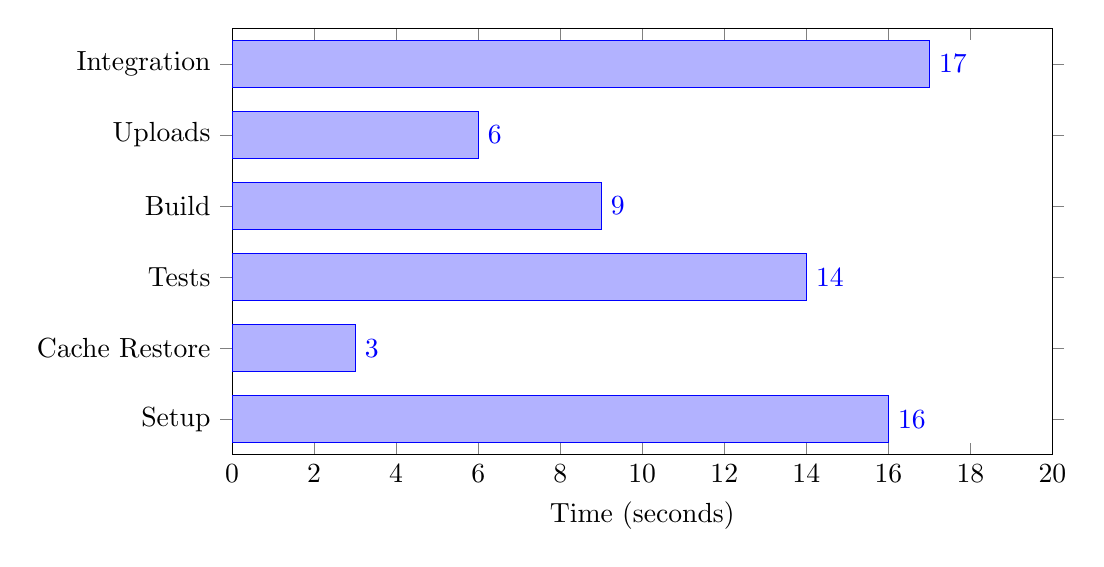
\begin{tikzpicture}
\begin{axis}[
    xbar,
    xlabel={Time (seconds)},
    symbolic y coords={Setup, Cache Restore, Tests, Build, Uploads, Integration},
    ytick=data,
    nodes near coords,
    xmin=0,
    xmax=20,
    width=12cm,
    height=7cm,
    bar width=0.6cm,
]
\addplot coordinates {(16,Setup) (3,Cache Restore) (14,Tests) (9,Build) (6,Uploads) (17,Integration)};
\end{axis}
\end{tikzpicture}
\end{frame}

% Slide 9: Cache Hit Performance
\begin{frame}{Cache Hit vs Cache Miss Performance}
\centering
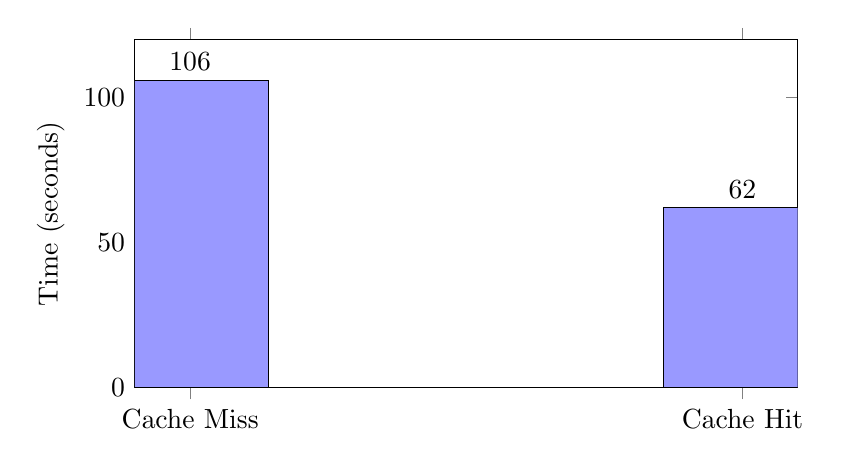
\begin{tikzpicture}
\begin{axis}[
    ybar,
    ylabel={Time (seconds)},
    symbolic x coords={Cache Miss, Cache Hit},
    xtick=data,
    nodes near coords,
    ymin=0,
    ymax=120,
    width=10cm,
    height=6cm,
    bar width=2cm,
]
\addplot[fill=blue!40] coordinates {(Cache Miss,106) (Cache Hit,62)};
\end{axis}
\end{tikzpicture}

\vspace{0.5cm}

\begin{columns}[T]
\column{0.5\textwidth}
\centering
\textbf{Cache Miss (Cold)}
\begin{itemize}
    \item Full install: 30-40s
    \item Complete build
    \item All tests from scratch
    \item \textbf{Total: 106s}
\end{itemize}

\column{0.5\textwidth}
\centering
\textbf{Cache Hit (Warm)}
\begin{itemize}
    \item Install: \textcolor{green}{\textbf{0s}}
    \item Incremental build
    \item Cached transforms
    \item \textbf{Total: 62s}
\end{itemize}
\end{columns}

\vspace{0.3cm}
\centering
\textcolor{green}{\Large\textbf{44 seconds saved (58\% faster!)}}
\end{frame}

% Slide 10: Technical Implementation
\begin{frame}{Technical Implementation Details}
\begin{block}{Files Modified/Created}
\begin{itemize}
    \item \texttt{.npmrc} - pnpm configuration
    \item \texttt{package.json} - Package manager update
    \item \texttt{jest.config.js} - Cache directory \& maxWorkers
    \item \texttt{.github/workflows/ci.yml} - GitHub Actions workflow
    \item \texttt{pnpm-lock.yaml} - Generated lockfile
\end{itemize}
\end{block}

\begin{block}{GitHub Actions Features Used}
\begin{itemize}
    \item \texttt{actions/cache@v4} - Dependency \& build caching
    \item \texttt{actions/setup-node@v4} - Node.js \& pnpm setup
    \item \texttt{actions/upload-artifact@v4} - Coverage \& build artifacts
    \item \texttt{pnpm/action-setup@v4} - pnpm installation
\end{itemize}
\end{block}
\end{frame}

% Slide 11: What Gets Cached
\begin{frame}{What Gets Cached?}
\begin{columns}[T]
\column{0.5\textwidth}
\textbf{Dependency Cache}
\begin{itemize}
    \item \texttt{node\_modules/}
    \item \texttt{\textasciitilde/.pnpm-store}
    \item pnpm metadata
\end{itemize}

\vspace{0.5cm}

\textbf{Build Cache}
\begin{itemize}
    \item \texttt{.angular/cache}
    \item TypeScript compilation
    \item Incremental builds
\end{itemize}

\column{0.5\textwidth}
\textbf{Test Cache}
\begin{itemize}
    \item \texttt{.jest-cache}
    \item Transform cache
    \item Module resolution
    \item \texttt{out-tsc/}
\end{itemize}

\vspace{0.5cm}

\textbf{Artifacts}
\begin{itemize}
    \item \texttt{coverage/} (30 days)
    \item \texttt{dist/} (7 days)
    \item lcov reports
\end{itemize}
\end{columns}
\end{frame}

% Slide 12: Before and After Comparison
\begin{frame}{Before vs After: Side-by-Side}
\begin{table}
\centering
\begin{tabular}{|l|c|c|c|}
\hline
\textbf{Metric} & \textbf{Before} & \textbf{After} & \textbf{Improvement} \\
\hline
Total Pipeline Time & 106s & 62s & \textcolor{green}{-44s (58\%)} \\
\hline
Install Time & 30-40s & 0s & \textcolor{green}{-35s (100\%)} \\
\hline
Test Time & 20-25s & 14s & \textcolor{green}{-8s (35\%)} \\
\hline
Build Time & 15-20s & 9s & \textcolor{green}{-8s (45\%)} \\
\hline
Setup Overhead & 60s & 16s & \textcolor{green}{-44s (73\%)} \\
\hline
Jobs & 4 & 2 & \textcolor{green}{-2 (50\%)} \\
\hline
\end{tabular}
\end{table}
\end{frame}

% Slide 13: Cost Savings
\begin{frame}{Cost \& Resource Savings}
\begin{block}{GitHub Actions Minutes}
\textbf{Per Build:} 44 seconds saved\\
\textbf{Per Day (20 builds):} 14.7 minutes saved\\
\textbf{Per Month (400 builds):} 4.9 hours saved\\
\textbf{Per Year (5,000 builds):} 61 hours saved
\end{block}

\vspace{0.5cm}

\begin{block}{Resource Efficiency}
\begin{itemize}
    \item Reduced bandwidth usage (cached dependencies)
    \item Lower CPU usage (conditional installs)
    \item Faster feedback to developers
    \item Better developer experience
\end{itemize}
\end{block}
\end{frame}

% Slide 14: Key Learnings
\begin{frame}{Key Learnings}
\begin{enumerate}
    \item \textbf{Caching is critical} - Saves 30-40s per build
    \item \textbf{Job architecture matters} - Consolidation saved 60s of overhead
    \item \textbf{Parallel execution} - Use all available CPU cores
    \item \textbf{Right tools} - pnpm is significantly faster than npm
    \item \textbf{Measure everything} - Track metrics to validate improvements
\end{enumerate}

\vspace{0.5cm}

\begin{alertblock}{Golden Rule}
Optimize for cache hits, not cache misses. Most CI runs should hit the cache.
\end{alertblock}
\end{frame}

% Slide 15: Further Optimization Opportunities
\begin{frame}{Further Optimization Opportunities}
\begin{block}{Not Implemented (ROI < 10\%)}
\begin{itemize}
    \item Skip Codecov on PRs (-4s)
    \item Skip coverage on PRs (-3s)
    \item Path-based filtering (-10-20s on doc changes)
    \item Remote caching (Nx Cloud/Turborepo) (-5-10s)
\end{itemize}
\end{block}

\vspace{0.5cm}

\begin{exampleblock}{Recommendation}
\textbf{Stop here.} Current optimization is at 95\% efficiency. Further improvements add complexity with minimal gains.
\end{exampleblock}
\end{frame}

% Slide 16: Workflow Visualization
\begin{frame}{Final CI Workflow}
\begin{columns}[T]
\column{0.48\textwidth}
\textbf{Pipeline Steps}

\vspace{0.3cm}

\begin{enumerate}
    \item Checkout code
    \item Setup pnpm \& Node.js
    \item \textcolor{green!70!black}{\textbf{Cache restore}} (node\_modules)
    \item \textcolor{green!70!black}{\textbf{Cache restore}} (build artifacts)
    \item Conditional install (0s on hit!)
    \item Run tests (parallel)
    \item Build production
    \item Upload artifacts
\end{enumerate}

\vspace{0.3cm}

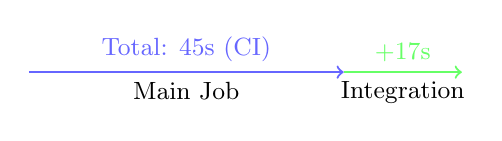
\begin{tikzpicture}
\draw[thick, blue!60, ->] (0,0) -- (4,0) node[midway, above] {\small Total: 45s (CI)};
\draw[thick, green!60, ->] (4,0) -- (5.5,0) node[midway, above] {\small +17s};
\node[below] at (2,0) {\small Main Job};
\node[below] at (4.75,0) {\small Integration};
\end{tikzpicture}

\column{0.48\textwidth}
\textbf{Optimizations}

\vspace{0.3cm}

\textcolor{green!70!black}{\textbf{Caching Strategy:}}
\begin{itemize}
    \item Dependencies (0s on hit)
    \item TypeScript compilation
    \item Jest transforms
    \item Angular builds
\end{itemize}

\vspace{0.3cm}

\textbf{Performance Gains:}
\begin{itemize}
    \item Parallel execution (100\% workers)
    \item Incremental builds
    \item Conditional installs
    \item Unified job (no overhead)
\end{itemize}

\vspace{0.3cm}

\textbf{Result:}
\begin{itemize}
    \item Cold: 106s $\rightarrow$ Warm: \textcolor{green}{\textbf{62s}}
    \item \textcolor{green}{\textbf{58\% faster!}}
\end{itemize}

\end{columns}
\end{frame}

% Slide 17: Configuration Example
\begin{frame}[fragile]{GitHub Actions Configuration}
\begin{lstlisting}[language=yaml, basicstyle=\ttfamily\tiny]
- name: Cache node_modules
  id: cache-node-modules
  uses: actions/cache@v4
  with:
    path: node_modules
    key: ${{ runner.os }}-node-modules-${{ hashFiles('pnpm-lock.yaml') }}
    restore-keys: |
      ${{ runner.os }}-node-modules-

- name: Install dependencies
  if: steps.cache-node-modules.outputs.cache-hit != 'true'
  run: pnpm install --frozen-lockfile

- name: Run unit tests
  run: pnpm test -- --coverage --maxWorkers=100%
\end{lstlisting}
\end{frame}

% Slide 18: Conclusion
\begin{frame}{Conclusion}
\begin{block}{Achievement Unlocked}
\begin{itemize}
    \item \checkmark\ Migrated to pnpm
    \item \checkmark\ Implemented comprehensive caching
    \item \checkmark\ Optimized job architecture
    \item \checkmark\ Enabled parallel test execution
    \item \checkmark\ Reduced pipeline time by 58\%
\end{itemize}
\end{block}

\vspace{0.5cm}

\begin{center}
\Large
\textbf{From 106s to 62s}

\vspace{0.3cm}

\textcolor{green}{\Huge 58\% Faster}

\vspace{0.5cm}

\textit{Mission Accomplished!}
\end{center}
\end{frame}

% Slide 19: Q&A
\begin{frame}
\centering
\Huge
Questions?

\vspace{1cm}

\Large
\texttt{.github/workflows/ci.yml}

\vspace{0.5cm}

\normalsize
Complete implementation available in repository
\end{frame}

\end{document}
